\documentclass{article}

\title{Flow-induced shape reconfiguration in houseplants}
\author{C Smith}
\date{\today}

\usepackage{siunitx}
\usepackage{graphicx}
\usepackage[round,authoryear]{natbib}
\bibliographystyle{apalike}
\usepackage[plain]{fancyref}
\usepackage{listings}
\lstset{
  basicstyle=\ttfamily}
\usepackage{amsmath,amsfonts,amssymb}

\begin{document}
\maketitle
\begin{abstract}
Write one paragraph here that explains what your report is about.
\end{abstract}

\section{Introduction}
Work from an inverted triangle (broader topics to more specific). Explain what you are interested, review some relevant literature, and then set up what your specific research question is. Cite literature using the author-year format, as in \citep{buck2020go}. If you need pictures to explain the relevant biomechanics, feel free to include. This section should also say a little why your research matters. 
% things to explain include drag, how it depends on speed, area, etc; why it matters to plants, what they can do to minimize or mitigate drag...
The last part of this section should be the specific hypotheses you seek to test. 

\section{Methods and materials}
Explain what you did, in enough detail so someone can replicate it. If you need pictures or drawings to explain the setup feel free to use them. 
% Need pictures! 

\subsection{Specimens and physical models}
\subsection{Drag measurements}
%\subsection{Statistical analyes}
Statistical analyses of the effects of both leaf and fan speed on drag and drag/area were performed using R \citep{r2020} using two-way analysis of variance (ANOVA); plots were prepared using the \lstinline{tidyverse} and \lstinline{ggplot2} libraries \citep{wickham2019tidyverse}. 

\section{Results}
%Explain factually what you found... leave interpretation of what it means for the final discussion section. Here you would include plots of what you found or comparison tables.
\Fref{fig:results1} shows... (what does it show). When the drag is normalized by area, the effect of leaf flexibility is apparent. \Fref{fig:results2} shows... (what does it show). 

\begin{figure}
\begin{center}
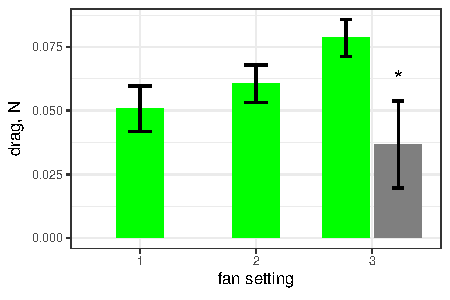
\includegraphics{data/results1.pdf}
\end{center}
\caption{Drag for grapefruit (green) and metal (gray) leaves at different fan speeds. The smaller model metal leaf has less drag than the actual grapefruit leaves because of smaller area (two-way ANOVA, $p<\num{1.67e-5}$, $n=5$).}
\label{fig:results1}
\end{figure}

\begin{figure}
\begin{center}
\includegraphics{data/results2.pdf}
\end{center}
\caption{Drag, normalized by area, for grapefruit (green) and metal (gray) leaves at different fan speeds. Normalized by area, the rigid metal leaf has significantly more drag than the flexible grapefruit leaves at low speeds and at the highest speed (two-way ANOVA, $p<0.003$, $n=5$).}
\label{fig:results2}
\end{figure}



\section{Discussion}
Here discuss what your results mean. Are your hypotheses supported or not? Do you have an answer to your overall research question?

\section{Acknowledgements}

% References
\bibliography{smith.bib}
\end{document}
